\chapter{Referencial Teórico}
\label{Referencial_Teorico}

\section{Internet das Coisas}%

A Internet das Coisas, do inglês \acf{IoT}, considerada um novo paradigma tecnológico, é uma extensão da internet atual, onde possibilita aos objetos do cotidiano, com capacidade computacional e de comunicação, conectar-se à Internet. Por meio dessa conexão é possível controlar remotamente os objetos, tornando-os provedores de serviços, assim fazendo-os objetos inteligentes \citep{Mancini2017}. Essa comunicação também viabiliza o registro contínuo de dados sobre o estado desses objetos durante o seu uso, mediante o uso de sensores, permitindo uma resposta aos dados recebidos, o que deixa visível a diferença básica de um objeto inteligente para um objeto qualquer conectado à Internet. 

O crescimento de IoT é exponencial. De acordo com \cite{Evan2011} é previsto que 50 (cinquenta) bilhões de dispositivos inteligentes estejam conectados à internet até 2020. Ao conectar objetos com diferentes recursos a uma rede, potencializa-se o surgimento de novas aplicações. Em IoT, os objetos podem prover comunicação entre usuários e dispositivos. Com isto emerge uma nova gama de aplicações tais como coleta de dados de pacientes e monitoramento de idosos, sensoriamento de ambientes de difícil acesso e inóspitos, pedágios inteligentes (através de chips com identificação por rafio frequência, veículos conseguem passar e pagar, sem precisar parar), relógios inteligentes (através de micro sensores, é possível medir batimentos cardíacos, pressão arterial e até qualidade do sono do usuário) entre outras \citep{Sundmaeker2010}. 


\section{Sistemas Web}%

A Web, que vem de \acf{WWW}, é um sistema distribuído que disponibiliza o acesso a serviços e/ou documentos por meio de uma rede. Um documento, o mesmo que uma página Web, é formada por objetos e um objeto se refere a um único arquivo. A maior parte da Web é escrita em linguagem \acf{HTML} que pode, dentro da sua estrutura, referenciar outros objetos, como por exemplo, imagens e vídeos, tornando sua construção mais dinâmica \citep{tanenbaum2008sistemas,kurose2014redesdecomputadores}. 

A arquitetura comumente usada em sistemas Web é a cliente-servidor, onde o servidor disponibiliza acesso aos documentos que podem ser solicitados por clientes, enquanto o cliente oferece uma interface amigável que torna a utilização desse serviço mais fácil para o usuário final, exemplificado na Figura \ref{fig:arquitetura-cliente-servidor}. O usuário acessa o browser, mais conhecido como navegador Web, e pode fazer as requisições por meio de uma referência chamada de \acf{URL}, que corresponde ao identificador uniforme de recurso. A URL identifica o documento ou objeto a ser chamado e através dela também é possível identificar o protocolo de transferência utilizada, com o uso do browser é possível também receber interações do usuário, podendo conter entrada de dados \citep{tanenbaum2008sistemas}.

\begin{figure}[ht]
    \centering
    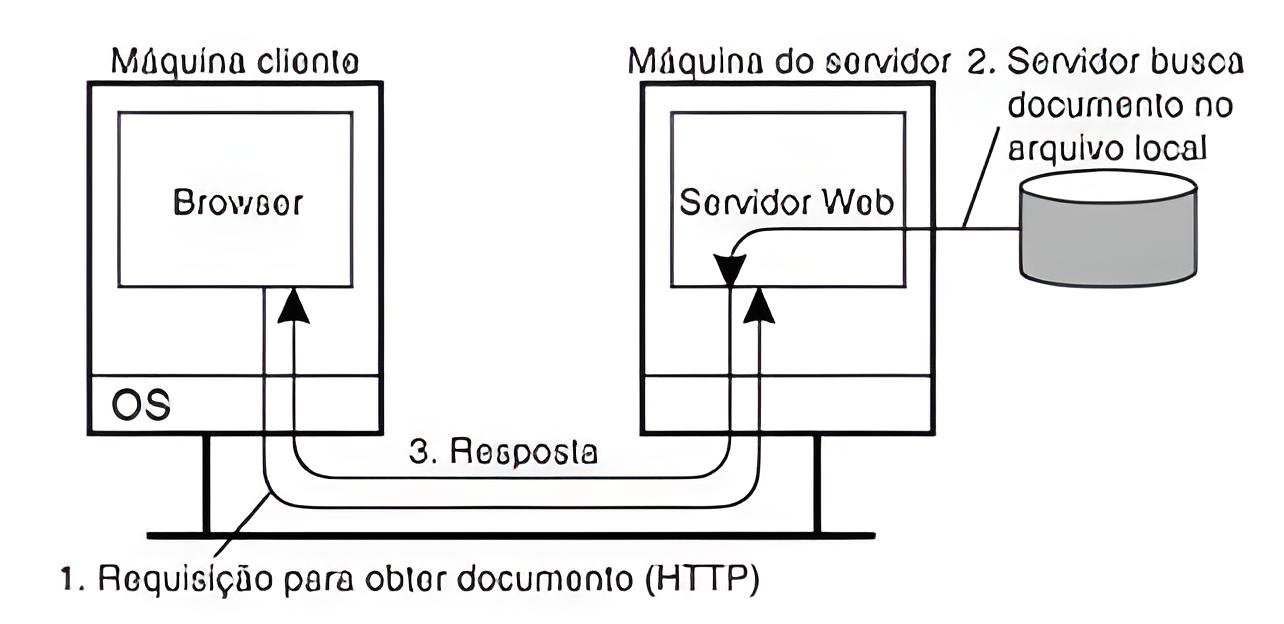
\includegraphics[width=10cm]{images/arquitetura-cliente-servidor.png}
    \caption{Organização Global de um site Web tradicional}
    \label{fig:arquitetura-cliente-servidor}
\end{figure}



\section{Módulo NodeMCU}%
    
\section{RFID}%

\section{Banco de Dados Relacional}%
    %Criar paragrafos sobre cada item
    %\subsection{Modelo Entidade Relacionamento}%
    %\subsection{SQL}%
    %\subsection{SGBD}%
    %\subsubsection{PostgreSQL}%
    
\section{Estado da Arte}%